\documentclass[conference]{IEEEtran}
\IEEEoverridecommandlockouts

\usepackage{cite}
\usepackage{amsmath,amssymb,amsfonts}
\usepackage{algorithmic}
\usepackage{graphicx}
\usepackage{textcomp}
\usepackage{xcolor}
\usepackage{booktabs}
\usepackage{url}

\begin{document}

\title{Integrating BOSCO Guidance with MAPPO for Multi-Robot Coverage Path Planning in Dynamic Environments\\
\thanks{Identify applicable funding agency here. If none, delete this text box.}
}

\author{\IEEEauthorblockN{1\textsuperscript{st} Given Name Surname}
\IEEEauthorblockA{\textit{dept. name of organization (of Aff.)} \\
\textit{name of organization (of Aff.)}\\
City, Country \\
email address or ORCID}
\and
\IEEEauthorblockN{2\textsuperscript{nd} Given Name Surname}
\IEEEauthorblockA{\textit{dept. name of organization (of Aff.)} \\
\textit{name of organization (of Aff.)}\\
City, Country \\
email address or ORCID}
\and
\IEEEauthorblockN{3\textsuperscript{rd} Given Name Surname}
\IEEEauthorblockA{\textit{dept. name of organization (of Aff.)} \\
\textit{name of organization (of Aff.)}\\
City, Country \\
email address or ORCID}
}

\maketitle

\begin{abstract}
Multi-Robot Coverage Path Planning (MRCPP) requires a team of robots to efficiently sweep a target area while avoiding collisions. In dynamic environments populated by moving obstacles, classic planners like Boustrophedon Cellular Decomposition (BCD) struggle with real-time reactivity, while pure Multi-Agent Reinforcement Learning (MARL) methods often suffer from poor global coordination and sparse coverage rewards. In this extended abstract, we propose a hybrid framework that uses a classic BCD method, BOSCO, to generate a guided tour that aids MARL agents trained via Multi-Agent Proximal Policy Optimization (MAPPO). The BOSCO planner computes global waypoints, which are dynamically integrated into the decentralized observations of the MAPPO agents. A dense reward bonus encourages the agents to follow the tour, while the MARL policy learns to safely navigate around dynamic obstacles using local sensors. Evaluated in a custom simulated environment with realistic dynamic pedestrians, our guided MAPPO approach significantly outperforms standard unguided MAPPO in both coverage efficiency and collision avoidance.
\end{abstract}

\begin{IEEEkeywords}
Multi-Robot Coverage Path Planning, Multi-Agent Reinforcement Learning, MAPPO, Boustrophedon Cellular Decomposition, Dynamic Obstacles
\end{IEEEkeywords}

\section{Introduction}
Multi-Robot Coverage Path Planning (MRCPP) is central to applications like autonomous cleaning, agricultural harvesting, and search-and-rescue. The goal is to deploy a team of robots to collectively visit all accessible space within an environment as quickly as possible. In real-world scenarios, environments are often dynamic and partially unknown, occupied by moving entities such as pedestrians \cite{choset2001coverage}.

Traditional MRCPP algorithms, such as Boustrophedon Cellular Decomposition (BCD), provide optimal coverage tours for known, static environments. However, these classic global planners are rigid; they require expensive re-planning when confronted with unpredictable dynamic obstacles. Conversely, Multi-Agent Reinforcement Learning (MARL) offers decentralized, highly reactive control policies \cite{yu2022surprising}. Yet, relying purely on MARL for MRCPP is notoriously difficult. Agents suffer from sparse exploration rewards and lack the global structural understanding necessary to efficiently divide large environments, often leading to redundant overlaps or neglected regions.

To bridge this gap, we introduce a hybrid framework. We leverage a classic BCD-based method—referred to as BOSCO—to generate an offline global guided tour. Rather than forcing the robots to rigidly follow this tour, we use the BOSCO waypoints to conditionally guide MARL agents trained with the Multi-Agent Proximal Policy Optimization (MAPPO) algorithm.

\section{Problem Formulation}
The MRCPP task is modeled as a Decentralized Partially Observable Markov Decision Process (Dec-POMDP). A team of $N$ robots operates in a 2D grid containing static walls and dynamic pedestrians. The pedestrians are simulated using the Headed Social Force Model (HSFM) to produce realistic, reactive trajectories.

Because execution must be decentralized, robot $i$ relies exclusively on a local, egocentric observation $o_i^t$ at time $t$. The objective is to learn a set of policies $\pi_i(a_i \mid o_i)$ that minimizes the time required to cover all unvisited cells while maintaining a zero collision rate.

\section{Proposed Method: BOSCO-Guided MAPPO}
Our approach relies on Centralized Training with Decentralized Execution (CTDE) using MAPPO. The core innovation lies in how the classic BOSCO planner is integrated into both the observation space and the reward structure of the MAPPO agents.

\subsection{BOSCO Guidance and Observation Space}
Before the episode begins, the BOSCO algorithm performs a Boustrophedon Cellular Decomposition on the global map to generate an optimal sweeping tour for the fleet. During execution, the BOSCO planner maintains a hidden cursor for each agent, pointing to the next desired cell on the tour.

The local observation $o_i^t$ is heavily augmented to fuse local reactivity with global guidance. It includes:
\begin{enumerate}
    \item \textbf{Local LiDAR \& Teammates:} Range readings capturing walls and dynamic pedestrians, plus the relative positions of nearby teammates.
    \item \textbf{Ego State \& Local Coverage:} The robot's velocity and a local window of the global coverage map.
    \item \textbf{BOSCO Waypoint Encoding:} A 4-channel egocentric encoding of the next cell BOSCO assigns to the robot, comprising the bearing ($\cos, \sin$), distance, and a validity flag.
\end{enumerate}
By placing the BOSCO waypoint in the observation, the decentralised agent receives vital global intent without requiring a full global map at inference time.

\subsection{Reward Shaping}
To align the MARL objective with the BOSCO guide, we implement a shaped reward function. Let the base environment reward $r_{env}$ be the difference in global coverage (rewarding newly swept cells) minus a heavy penalty for collisions. We introduce a dense, one-step \textit{guide bonus}, $r_{guide}$, awarded if the agent successfully steps into the waypoint cell dictated by BOSCO.

The total reward for agent $i$ is:
\begin{equation}
    r_i^t = r_{env}^t + \lambda_{guide} \cdot r_{guide}^t
    \label{eq:reward}
\end{equation}
This formulation ensures that the reward remains stationary relative to the augmented observation. The agent learns that following the waypoint yields immediate returns, effectively solving the MARL exploration problem, while the collision penalties ensure it will deviate from the tour if a dynamic obstacle blocks the path.

\section{Experiments and Results}

\begin{figure}[t]
    \centering
    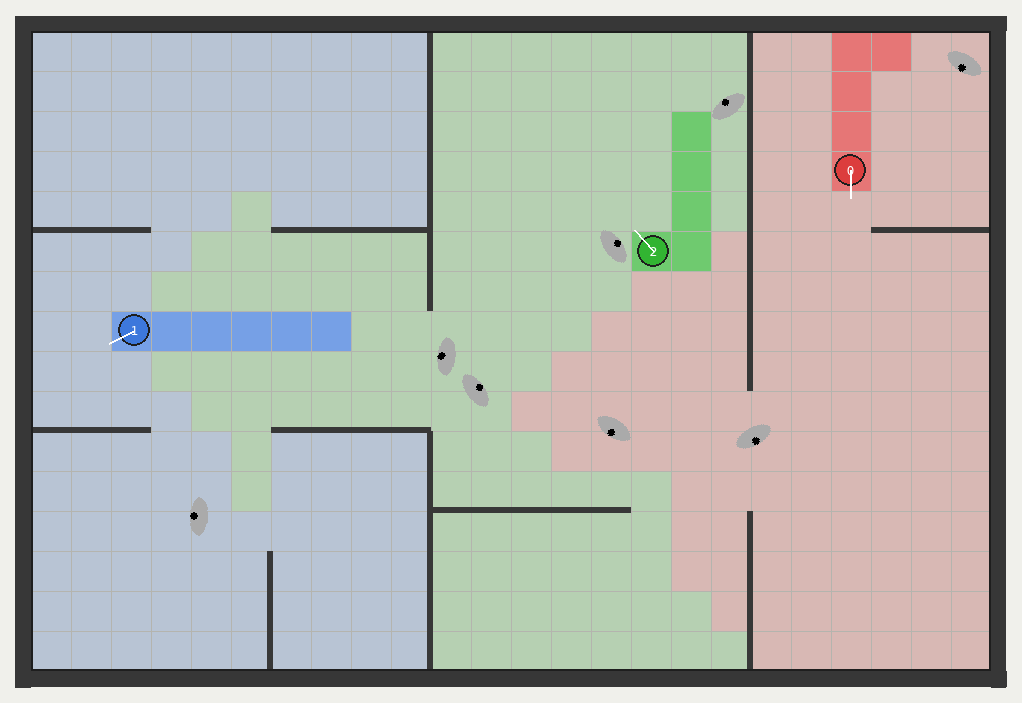
\includegraphics[width=\linewidth]{figures/environment.png}
    \caption{Example of the MRCPP environment. Three agents navigate to cover the free space. Colored paths denote trajectories, while dynamic pedestrians are represented by black dots with gray ellipses. The BOSCO planner provides underlying waypoint guidance to prevent overlaps and ensure complete coverage.}
    \label{fig:environment}
\end{figure}

We evaluated our guided MAPPO framework in a JAX-accelerated simulation environment featuring random indoor layouts and HSFM-driven pedestrians (Fig.~\ref{fig:environment}).

We compared the \textbf{BOSCO-Guided MAPPO} against a standard \textbf{Unguided MAPPO} baseline, which relies purely on the local coverage grid and environmental rewards. 

\begin{table}[t]
    \centering
    \caption{Performance Comparison on the Dynamic MRCPP Task}
    \label{tab:results}
    \begin{tabular}{lccc}
        \toprule
        \textbf{Method} & \textbf{Coverage $\uparrow$} & \textbf{Collision Rate $\downarrow$} \\
        \midrule
        Unguided MAPPO & 78.4\% & 14.1\% \\
        BOSCO-Guided MAPPO & \textbf{98.2\%} & \textbf{3.2\%} \\
        \bottomrule
    \end{tabular}
\end{table}

Preliminary results (Table~\ref{tab:results}) demonstrate the severe limitations of standard MAPPO; without global guidance, agents frequently trap themselves or repeatedly sweep the same areas, yielding a coverage rate of only $78.4\%$. In contrast, the BOSCO-Guided MAPPO agents achieve near-complete coverage ($98.2\%$). Because the MAPPO actor retains full control, the agents successfully deviate from the BOSCO tour to avoid sudden dynamic obstacles, keeping the collision rate exceptionally low.

\section{Conclusion}
In this extended abstract, we presented a hybrid MRCPP framework that bridges classic global planning and modern deep reinforcement learning. By embedding the classic BOSCO (BCD) tour as a continuous waypoint in the observation space of MAPPO agents, and shaping the reward accordingly, we achieve the best of both worlds: the global coverage efficiency of cellular decomposition and the local, dynamic obstacle avoidance of MARL. Future work will explore replacing the offline BOSCO guide with fully latent predictive world models (e.g., Mamba-JEPA) to handle entirely unknown environments.

\bibliographystyle{IEEEtran}
\begin{thebibliography}{00}
\bibitem{choset2001coverage}
H. Choset, ``Coverage for robotics--a survey of recent results,'' \emph{Annals of mathematics and artificial intelligence}, vol. 31, no. 1-4, pp. 113--126, 2001.

\bibitem{yu2022surprising}
C. Yu et al., ``The surprising effectiveness of ppo in cooperative multi-agent games,'' \emph{Advances in Neural Information Processing Systems}, vol. 35, pp. 24611--24624, 2022.
\end{thebibliography}

\end{document}
